%%==========================================================================%%
%% Author : Abascal Fern�ndez, Patricia                                     %%
%% Author : S�nchez Barreiro, Pablo                                         %%
%% Version: 1.2, 23/04/2013                                                 %%
%%                                                                          %%
%% Memoria del Proyecto Fin de Carrera                                      %%
%% Domain Engineering/Ejemplo de Generaci�n de C�digo C#: Caso Complejo     %%
%%==========================================================================%%
Antes de comenzar a exponer los ejemplos m�s complejo, vamos a introducir aquellos conceptos que pasamos por algo en la secci�n \ref{domain:sec:transf} dada su complejidad: las relaciones bidireccionales y la herencia m�ltiple.

 \paragraph{Relaciones Bidireccionales} \ \\
 \begin{figure}[!tb]
  \centering
  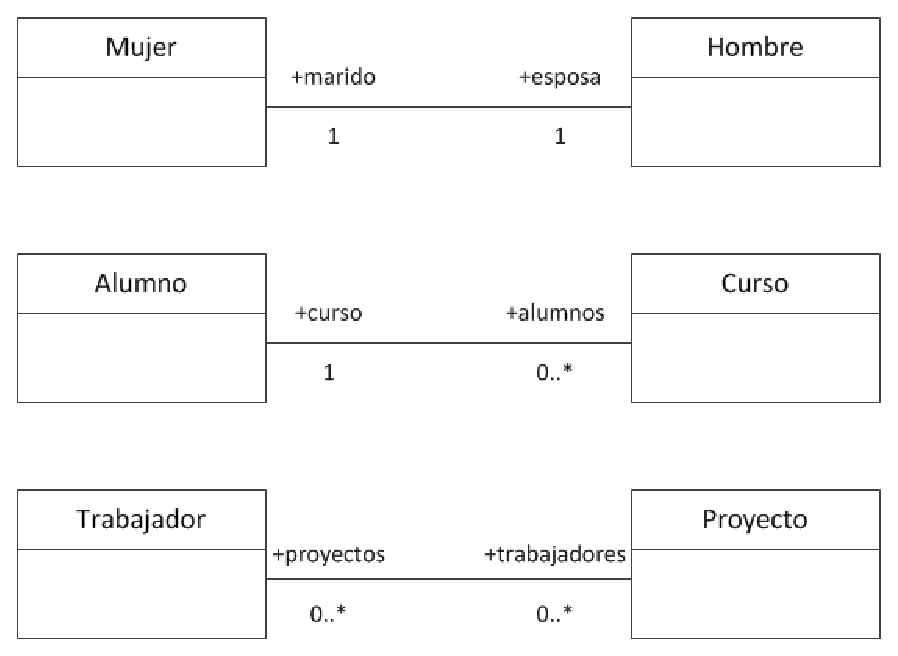
\includegraphics[width=.75\linewidth]{domainEngineering/images/bidireccionales.eps} \\
  \caption{Tipos de relaciones bidireccionales}
  \label{dom:fig:bid}
\end{figure}

Las relaciones bidireccionales son aquellas en las que ambas clases relacionadas disponen de atributos de la clase opuesta. Existen tres tipos de relaciones bidireccionales:
 \begin{itemize}
   \item \emph{Bidireccionalidad one to one}, en las que cada clase recibe un elemento de la clase opuesta (figura \ref{dom:fig:bid}, Mujer-Marido).
   \item \emph{Bidireccionalidad one to many}, en la que una de las clases recibe un elemento de la clase destino y la otra recibe una colecci�n de elementos de la clase opuesta (figura \ref{dom:fig:bid}, Alumno-Curso).
   \item \emph{Bidireccionalidad many to many}, en la que ambas clases reciben colecciones de la clase opuesta (figura \ref{dom:fig:bid}, Trabajadores-Proyectos).
 \end{itemize}

 Llegados a este punto, bas�ndonos en los ejemplos de la figura \ref{dom:fig:bid} nos surgen algunas preguntas:
 \begin{enumerate}
   \item �Si una mujer A tiene un esposo B y ese esposo B tiene una mujer que no sea A?
   \item �Si un alumno tiene asignado un curso pero ese curso no tiene a dicho alumno en su lista de alumnado?
   \item �Si un trabajador tiene asignado un proyecto pero en el listado de trabajadores dicho trabajador no aparece?
 \end{enumerate}
�Existe alguna forma de poner soluci�n a estos problemas?, la respuesta es s�, a la hora de tratar este tipo de relaciones bidireccionales en los generadores de c�digo correspondientes no basta con generar las propiedades tal como hemos estado haciendo hasta ahora sino que debemos implementar las propiedades a generar de una forma cuidadosa y exhaustiva para que no se produzcan este tipo de incoherencias, incluso recurriendo a la creaci�n de m�todos adicionales. Veamos a grandes rasgos en la tabla \ref{dom:table:bid} c�mo ser�a la implementaci�n de la relaci�n bidireccional one to one:
\begin{table}%
\begin{tabularx}{15cm}{|l|X|X|}
 \hline
{}&{\textbf{Mujer soltera}}&{\textbf{Mujer casada}} \\ \hline
{\textbf{Hombre soltero}} &
                Se casan el hombre soltero y la mujer soltera.
&  La mujer casada se divorcia. El antiguo marido de la mujer divorciada queda soltero. La mujer divorciada y el hombre soltero se casan. \\ \hline
{\textbf{Hombre casado}} & El hombre casado se divorcia. La antigua mujer del marido divorciado queda soltera. Se casan la mujer soltera y el hombre divorciado.
& El hombre casado se divorcia. La antigua mujer del marido divorciado queda soltera. La mujer casada se divorcia. El antiguo marido de la mujer divorciada queda soltero. Se casan la mujer divorciada y el hombre divorciado. \\ \hline
\end{tabularx}
\caption{Soluci�n para evitar incoherencias en el c�digo C\# en la bidireccionalidad one to one}
\label{dom:table:bid}
\end{table}%
El siguiente paso ser�a pasar dicha tabla a c�digo C\# y comprobar que funciona correctamente. Se sigue un proceso an�logo para el resto de relaciones bidireccionales.

\paragraph{Herencia m�ltiple} \ \\

\begin{figure}[!tb]
  \centering
  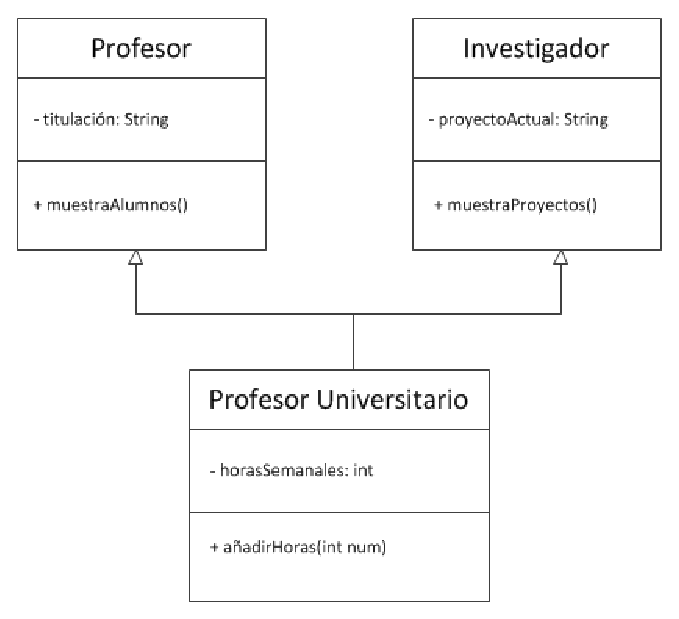
\includegraphics[width=.50\linewidth]{domainEngineering/images/herenciamultiple.eps} \\
  \caption{Tipos de relaciones bidireccionales}
  \label{dom:fig:her}
\end{figure}

